\documentclass[crop,tikz]{standalone}% 'crop' is the default for v1.0, before it was 'preview'
%\usetikzlibrary{...}% tikz package already loaded by 'tikz' option
\usepackage{circuitikz}
%answer from Qrrbrbirlbel for https://tex.stackexchange.com/questions/134067/circuitikz-wire-kink-thingy-when-wires-cross
\tikzset{
  declare function={% in case of CVS which switches the arguments of atan2
    atan3(\a,\b)=ifthenelse(atan2(0,1)==90, atan2(\a,\b), atan2(\b,\a));},
  kinky cross radius/.initial=+.125cm,
  @kinky cross/.initial=+, kinky crosses/.is choice,
  kinky crosses/left/.style={@kinky cross=-},kinky crosses/right/.style={@kinky cross=+},
  kinky cross/.style args={(#1)--(#2)}{
    to path={
      let \p{@kc@}=($(\tikztotarget)-(\tikztostart)$),
          \n{@kc@}={atan3(\p{@kc@})+180} in
      -- ($(intersection of \tikztostart--{\tikztotarget} and #1--#2)!%
             \pgfkeysvalueof{/tikz/kinky cross radius}!(\tikztostart)$)
      arc [ radius     =\pgfkeysvalueof{/tikz/kinky cross radius},
            start angle=\n{@kc@},
            delta angle=\pgfkeysvalueof{/tikz/@kinky cross}180 ]
      -- (\tikztotarget)}}}

\begin{document}
\usetikzlibrary{shapes,snakes}
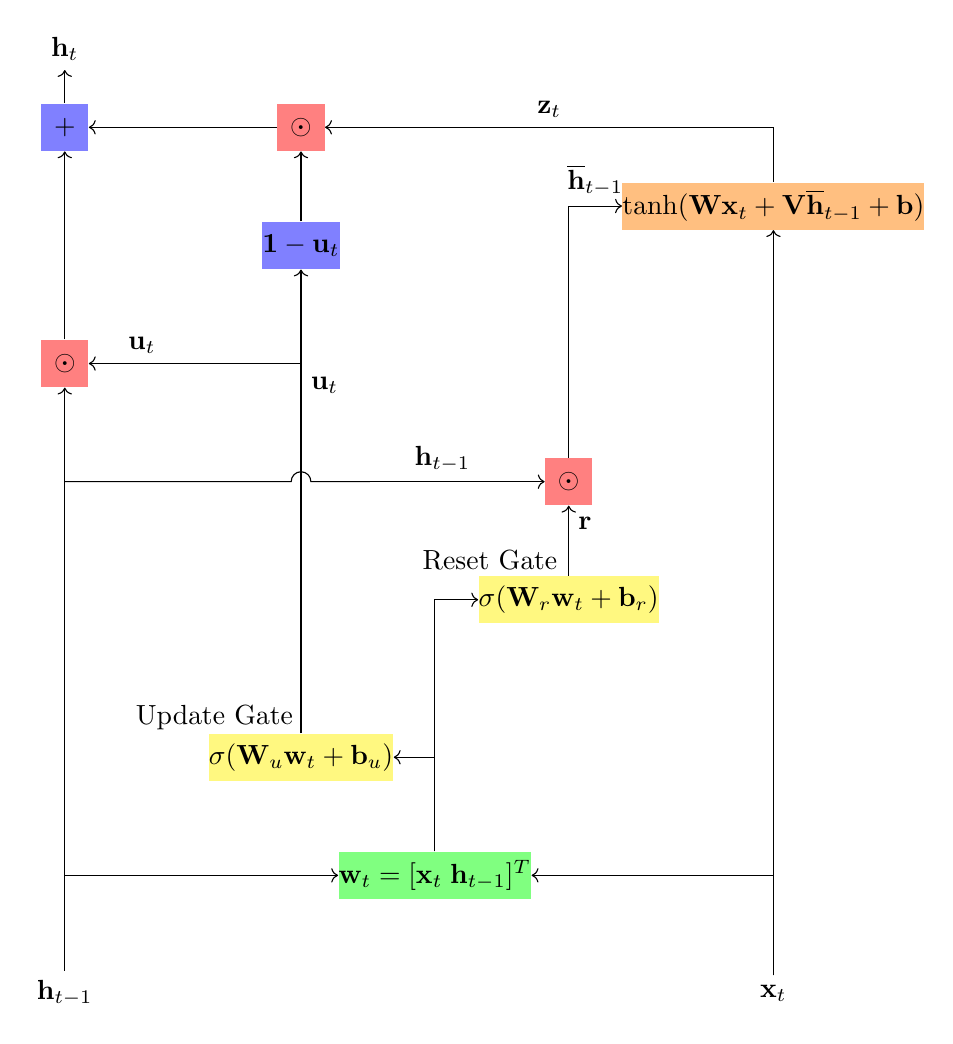
\begin{tikzpicture}
\tikzstyle{gate}=[rectangle,fill=yellow!50,minimum size=17pt,inner sep=0pt]
\tikzstyle{tanGate}=[rectangle,fill=orange!50,minimum size=17pt,inner sep=0pt]
\tikzstyle{fun}=[ellipse,fill=orange!50,minimum size=17pt,inner sep=0pt]
\tikzstyle{merge}=[rectangle,fill=green!50,minimum size=17pt,inner sep=0pt]
\tikzstyle{times}=[rectangle,fill=red!50,minimum size=17pt,inner sep=0pt]
\tikzstyle{plus}=[rectangle,fill=blue!50,minimum size=17pt,inner sep=0pt]

%get labels.
\node at (1.9,2.5) {Update Gate};
\node at (5.4,4.5) {Reset Gate};

\node(hOld) at (0,-1) {$\mathbf{h}_{t-1}$};
\node(x)    at (9,-1) {$\mathbf{x}_t$};

\node[merge] (mergeW) at (4.7,0.5) {$\mathbf{w}_t = [\mathbf{x}_t \; \mathbf{h}_{t-1}]^T$};
\draw[->] (x) |- (mergeW);
\draw[->] (hOld) |- (mergeW);

\node[gate] (rSig) at (3,2) {$\sigma(\mathbf{W}_u \mathbf{w}_t + \mathbf{b}_u)$};
\node[gate] (hSig) at (6.4,4) {$\sigma(\mathbf{W}_r \mathbf{w}_t + \mathbf{b}_r)$};

\draw[->] (mergeW) |-  (rSig);
\draw[->] (mergeW) |-  (hSig);

\node[times] (rMul) at (6.4,5.5) {$\odot$};
\node (endht) at (4,5.5) {};
\node (startht) at (0, 5.5) {};
\node (endu) at (3,7) {};
\draw[->] (3.5,5.5) -- (rMul)node[pos=0.5, above] {$\mathbf{h}_{t-1}$};

\draw (0, 5.5) to [kinky cross=(rSig)--(endu), kinky crosses=left] (endht);


\draw[->] (hSig) -- (rMul) node[near end, below, right] {$\mathbf{r}$};
\node[tanGate] (hBar) at (9,9) {$\tanh(\mathbf{W} \mathbf{x}_t + \mathbf{V}\overline{\mathbf{h}}_{t-1} + \mathbf{b})$};
\draw[->] (x) -- (hBar);
\draw[->] (rMul) |- (hBar) node[near end, above] {$\overline{\mathbf{h}}_{t-1}$};

\node[plus] (invR) at (3,8.5) {$\mathbf{1} - \mathbf{u}_t$};

\node[times] (rtimeshOld) at (0,7) {$\odot$};
\draw[->] (rSig) -- (3,7) -- (rtimeshOld) node[near end, above] {$\mathbf{u}_t$};
\draw[->] (hOld) -- (rtimeshOld);

\node[times] (hBarTimesrt) at (3,10) {$\odot$};
\draw[->] (rSig) -- (invR) node[near end, right] {$\mathbf{u}_t$};
\draw[->] (invR) -- (hBarTimesrt);
\draw[->] (hBar) |- (hBarTimesrt) node[near end, above] {$\mathbf{z}_t$};


% \draw[->] (iSig) -- (ctBarTimesIt) node[near end, left] {$\mathbf{i}_t$};
% \draw[->] (ctBar) |- (ctBarTimesIt) node[near end, above] {$\bar{\mathbf{s}}_t$};

\node[plus] (compht) at (0,10) {$+$};
\draw[->] (rtimeshOld) -- (compht);
\draw[->] (hBarTimesrt) -- (compht);


\node (ht) at (0,11) {$\mathbf{h}_t$};
\draw[->] (compht) -- (ht);



\end{tikzpicture}
\end{document}
